
%----------------------------------------------------------------
%
%  File    :  reif_fuer_insel_jrnl.tex
%
%  Authors :  Voglsam, Magin, Eisenhut
% 
%  Created :  6 Sept 2019
% 
%  Changed :  7 Sept 2019
% 
%---------------------------------------------------------------

% *** Authors should verify (and, if needed, correct) their LaTeX system  ***
% *** with the testflow diagnostic prior to trusting their LaTeX platform ***
% *** with production work. The IEEE's font choices and paper sizes can   ***
% *** trigger bugs that do not appear when using other class files.       ***                          ***
% The testflow support page is at:
% http://www.michaelshell.org/tex/testflow/

\documentclass[journal]{IEEEtran}
%----------------Praeambel----------------
\usepackage[english, ngerman]{babel}
%Hauptsprache Deutsch, auch Englisch
\usepackage[center]{caption}
%Bildbeschriftung zentriert
%----------------Grafiken---------------
\ifCLASSINFOpdf
 \usepackage[pdftex]{graphicx}
 % declare the path(s) where your graphic files are
 \graphicspath{{images/}}
 % declare extensions so you won't have to specify these with
 % every instance of \includegraphics
 \DeclareGraphicsExtensions{.pdf,.jpeg,.png, .JPG}
\else
 % or other class option (dvipsone, dvipdf, if not using dvips). graphicx
 % will default to the driver specified in the system graphics.cfg if no
 % driver is specified.
 \usepackage[dvips]{graphicx}
 % declare extensions so you won't have to specify these with
 % every instance of \includegraphics
\DeclareGraphicsExtensions{.eps}
\fi
\usepackage{float}
%um [H] bei \usepackage{float}[H] verwenden zu können: Bild ist exakt an dieser Stelle
%----------------Grafiken Ende---------------
%----------Literaturverzeichnis----------
\usepackage{cite}

%Zitierpackage
%\bibliographystyle{IEEEtran}
%liefert den richtigen style für IEEE
%\bibliography{reif_fuer_die_insel_jrnl}
%an dieser Stelle wird das Literaturverzeichnis eingefügt
%\label{app:literatur}
%Referenz für Literaturverzeichnis
%---Automatisches Literaturverzweichnis---
%-JabRef herunterladen
%Datei/Bibliothek öffnen anklicken
%Auswählen: "\Gruppenarbeit_4\Reif_fuer_die_Insel\reif_fuer_die_insel_jrnl.bib"
%-TeXstudio
%Optionen/TeXstudio Konfigurieren/Erzeugen:
%li unten "Erweiterte Optionen" auswählen mit Hackerl
%Bei Erzeugen/Standardcompiler "MakeIndex" hinzufügen (Button konfigurieren)
%Bei BenutzebBefehle
% makeindex.exe "reif_fuer_die_insel_jrnl".nlo -s nomencl.ist -o "reif_fuer_die_insel_jrnl".nls
%hinzufügen. Damit wird aus bib ein bbl
%---Automatisches Literaturverzweichnis Ende---
%----------Literaturverzeichnis Ende----------
% ----------Abkürzungsverzeichnis----------
% Quelle: https://strobelstefan.org/?p=153
\usepackage{nomencl}
% Befehl umbenennen in abk
\let\abk\nomenclature
% Deutsche Überschrift
\renewcommand{\nomname}{Abkürzungsverzeichnis}
%Zeilenlaenge
\setlength{\nomlabelwidth}{.20\hsize}
% Punkte zw. Abkürzung und Erklärung
\renewcommand{\nomlabel}[1]{#1 \dotfill}
% Zeilenabstände verkleinern
\setlength{\nomitemsep}{-\parsep}
\makenomenclature
% Beispiel: Fachhochschule Campus Wien (FHCW)\abk{FHCW}{Fachhochschule Campus Wien}
%----------Abkürzungsverzeichnis Ende----------
\usepackage{nameref}
\usepackage{hyperref}


%%von julian hinzugefügt


%Referenzen die verlinkt sind Immer letzter \usepackage Eintrag!!!
%---------------Praeambel Ende----------------


% Some very useful LaTeX packages include:
% (uncomment the ones you want to load)

% *** CITATION PACKAGES ***
%
%\usepackage{cite}
% cite.sty was written by Donald Arseneau
% V1.6 and later of IEEEtran pre-defines the format of the cite.sty package
% \cite{} output to follow that of the IEEE. Loading the cite package will
% result in citation numbers being automatically sorted and properly
% "compressed/ranged". e.g., [1], [9], [2], [7], [5], [6] without using
% cite.sty will become [1], [2], [5]--[7], [9] using cite.sty. cite.sty's
% \cite will automatically add leading space, if needed. Use cite.sty's
% noadjust option (cite.sty V3.8 and later) if you want to turn this off
% such as if a citation ever needs to be enclosed in parenthesis.
% cite.sty is already installed on most LaTeX systems. Be sure and use
% version 5.0 (2009-03-20) and later if using hyperref.sty.
% The latest version can be obtained at:
% http://www.ctan.org/pkg/cite
% The documentation is contained in the cite.sty file itself.

% *** GRAPHICS RELATED PACKAGES ***
%
\ifCLASSINFOpdf
  % \usepackage[pdftex]{graphicx}
  % declare the path(s) where your graphic files are
  % \graphicspath{{../pdf/}{../jpeg/}}
  % and their extensions so you won't have to specify these with
  % every instance of \includegraphics
  % \DeclareGraphicsExtensions{.pdf,.jpeg,.png}
\else
  % or other class option (dvipsone, dvipdf, if not using dvips). graphicx
  % will default to the driver specified in the system graphics.cfg if no
  % driver is specified.
  % \usepackage[dvips]{graphicx}
  % declare the path(s) where your graphic files are
  % \graphicspath{{../eps/}}
  % and their extensions so you won't have to specify these with
  % every instance of \includegraphics
  % \DeclareGraphicsExtensions{.eps}
\fi
% graphicx was written by David Carlisle and Sebastian Rahtz. It is
% required if you want graphics, photos, etc. graphicx.sty is already
% installed on most LaTeX systems. The latest version and documentation
% can be obtained at: 
% http://www.ctan.org/pkg/graphicx
% Another good source of documentation is "Using Imported Graphics in
% LaTeX2e" by Keith Reckdahl which can be found at:
% http://www.ctan.org/pkg/epslatex
%
% latex, and pdflatex in dvi mode, support graphics in encapsulated
% postscript (.eps) format. pdflatex in pdf mode supports graphics
% in .pdf, .jpeg, .png and .mps (metapost) formats. Users should ensure
% that all non-photo figures use a vector format (.eps, .pdf, .mps) and
% not a bitmapped formats (.jpeg, .png). The IEEE frowns on bitmapped formats
% which can result in "jaggedy"/blurry rendering of lines and letters as
% well as large increases in file sizes.
%
% You can find documentation about the pdfTeX application at:
% http://www.tug.org/applications/pdftex

% *** MATH PACKAGES ***
%
%\usepackage{amsmath}
% A popular package from the American Mathematical Society that provides
% many useful and powerful commands for dealing with mathematics.
%
% Note that the amsmath package sets \interdisplaylinepenalty to 10000
% thus preventing page breaks from occurring within multiline equations. Use:
%\interdisplaylinepenalty=2500
% after loading amsmath to restore such page breaks as IEEEtran.cls normally
% does. amsmath.sty is already installed on most LaTeX systems. The latest
% version and documentation can be obtained at:
% http://www.ctan.org/pkg/amsmath

% *** SPECIALIZED LIST PACKAGES ***
%
%\usepackage{algorithmic}
% algorithmic.sty was written by Peter Williams and Rogerio Brito.
% This package provides an algorithmic environment fo describing algorithms.
% You can use the algorithmic environment in-text or within a figure
% environment to provide for a floating algorithm. Do NOT use the algorithm
% floating environment provided by algorithm.sty (by the same authors) or
% algorithm2e.sty (by Christophe Fiorio) as the IEEE does not use dedicated
% algorithm float types and packages that provide these will not provide
% correct IEEE style captions. The latest version and documentation of
% algorithmic.sty can be obtained at:
% http://www.ctan.org/pkg/algorithms
% Also of interest may be the (relatively newer and more customizable)
% algorithmicx.sty package by Szasz Janos:
% http://www.ctan.org/pkg/algorithmicx

% *** ALIGNMENT PACKAGES ***
%
%\usepackage{array}
% Frank Mittelbach's and David Carlisle's array.sty patches and improves
% the standard LaTeX2e array and tabular environments to provide better
% appearance and additional user controls. As the default LaTeX2e table
% generation code is lacking to the point of almost being broken with
% respect to the quality of the end results, all users are strongly
% advised to use an enhanced (at the very least that provided by array.sty)
% set of table tools. array.sty is already installed on most systems. The
% latest version and documentation can be obtained at:
% http://www.ctan.org/pkg/array

% IEEEtran contains the IEEEeqnarray family of commands that can be used to
% generate multiline equations as well as matrices, tables, etc., of high
% quality.

% *** SUBFIGURE PACKAGES ***
%\ifCLASSOPTIONcompsoc
%  \usepackage[caption=false,font=normalsize,labelfont=sf,textfont=sf]{subfig}
%\else
%  \usepackage[caption=false,font=footnotesize]{subfig}
%\fi
% subfig.sty, written by Steven Douglas Cochran, is the modern replacement
% for subfigure.sty, the latter of which is no longer maintained and is
% incompatible with some LaTeX packages including fixltx2e. However,
% subfig.sty requires and automatically loads Axel Sommerfeldt's caption.sty
% which will override IEEEtran.cls' handling of captions and this will result
% in non-IEEE style figure/table captions. To prevent this problem, be sure
% and invoke subfig.sty's "caption=false" package option (available since
% subfig.sty version 1.3, 2005/06/28) as this is will preserve IEEEtran.cls
% handling of captions.
% Note that the Computer Society format requires a larger sans serif font
% than the serif footnote size font used in traditional IEEE formatting
% and thus the need to invoke different subfig.sty package options depending
% on whether compsoc mode has been enabled.
%
% The latest version and documentation of subfig.sty can be obtained at:
% http://www.ctan.org/pkg/subfig

% *** FLOAT PACKAGES ***
%
%\usepackage{fixltx2e}
% fixltx2e, the successor to the earlier fix2col.sty, was written by
% Frank Mittelbach and David Carlisle. This package corrects a few problems
% in the LaTeX2e kernel, the most notable of which is that in current
% LaTeX2e releases, the ordering of single and double column floats is not
% guaranteed to be preserved. Thus, an unpatched LaTeX2e can allow a
% single column figure to be placed prior to an earlier double column
% figure.
% Be aware that LaTeX2e kernels dated 2015 and later have fixltx2e.sty's
% corrections already built into the system in which case a warning will
% be issued if an attempt is made to load fixltx2e.sty as it is no longer
% needed.
% The latest version and documentation can be found at:
% http://www.ctan.org/pkg/fixltx2e

%\usepackage{stfloats}
% stfloats.sty was written by Sigitas Tolusis. This package gives LaTeX2e
% the ability to do double column floats at the bottom of the page as well
% as the top. (e.g., "\begin{figure*}[!b]" is not normally possible in
% LaTeX2e). It also provides a command:
%\fnbelowfloat
% to enable the placement of footnotes below bottom floats (the standard
% LaTeX2e kernel puts them above bottom floats). This is an invasive package
% which rewrites many portions of the LaTeX2e float routines. It may not work
% with other packages that modify the LaTeX2e float routines. The latest
% version and documentation can be obtained at:
% http://www.ctan.org/pkg/stfloats
% Do not use the stfloats baselinefloat ability as the IEEE does not allow
% \baselineskip to stretch. Authors submitting work to the IEEE should note
% that the IEEE rarely uses double column equations and that authors should try
% to avoid such use. Do not be tempted to use the cuted.sty or midfloat.sty
% packages (also by Sigitas Tolusis) as the IEEE does not format its papers in
% such ways.
% Do not attempt to use stfloats with fixltx2e as they are incompatible.
% Instead, use Morten Hogholm'a dblfloatfix which combines the features
% of both fixltx2e and stfloats:
%
% \usepackage{dblfloatfix}
% The latest version can be found at:
% http://www.ctan.org/pkg/dblfloatfix

%\ifCLASSOPTIONcaptionsoff
%  \usepackage[nomarkers]{endfloat}
% \let\MYoriglatexcaption\caption
% \renewcommand{\caption}[2][\relax]{\MYoriglatexcaption[#2]{#2}}
%\fi
% endfloat.sty was written by James Darrell McCauley, Jeff Goldberg and 
% Axel Sommerfeldt. This package may be useful when used in conjunction with 
% IEEEtran.cls'  captionsoff option. Some IEEE journals/societies require that
% submissions have lists of figures/tables at the end of the paper and that
% figures/tables without any captions are placed on a page by themselves at
% the end of the document. If needed, the draftcls IEEEtran class option or
% \CLASSINPUTbaselinestretch interface can be used to increase the line
% spacing as well. Be sure and use the nomarkers option of endfloat to
% prevent endfloat from "marking" where the figures would have been placed
% in the text. The two hack lines of code above are a slight modification of
% that suggested by in the endfloat docs (section 8.4.1) to ensure that
% the full captions always appear in the list of figures/tables - even if
% the user used the short optional argument of \caption[]{}.
% IEEE papers do not typically make use of \caption[]'s optional argument,
% so this should not be an issue. A similar trick can be used to disable
% captions of packages such as subfig.sty that lack options to turn off
% the subcaptions:
% For subfig.sty:
% \let\MYorigsubfloat\subfloat
% \renewcommand{\subfloat}[2][\relax]{\MYorigsubfloat[]{#2}}
% However, the above trick will not work if both optional arguments of
% the \subfloat command are used. Furthermore, there needs to be a
% description of each subfigure *somewhere* and endfloat does not add
% subfigure captions to its list of figures. Thus, the best approach is to
% avoid the use of subfigure captions (many IEEE journals avoid them anyway)
% and instead reference/explain all the subfigures within the main caption.
% The latest version of endfloat.sty and its documentation can obtained at:
% http://www.ctan.org/pkg/endfloat
%
% The IEEEtran \ifCLASSOPTIONcaptionsoff conditional can also be used
% later in the document, say, to conditionally put the References on a 
% page by themselves.

% *** PDF, URL AND HYPERLINK PACKAGES ***
%
%\usepackage{url}
% url.sty was written by Donald Arseneau. It provides better support for
% handling and breaking URLs. url.sty is already installed on most LaTeX
% systems. The latest version and documentation can be obtained at:
% http://www.ctan.org/pkg/url
% Basically, \url{my_url_here}.

% *** Do not adjust lengths that control margins, column widths, etc. ***
% *** Do not use packages that alter fonts (such as pslatex).         ***
% There should be no need to do such things with IEEEtran.cls V1.6 and later.
% (Unless specifically asked to do so by the journal or conference you plan
% to submit to, of course. )


% correct bad hyphenation here
\hyphenation{mobil-funk-netz share}


\begin{document}
%
% paper title
% Titles are generally capitalized except for words such as a, an, and, as,
% at, but, by, for, in, nor, of, on, or, the, to and up, which are usually
% not capitalized unless they are the first or last word of the title.
% Linebreaks \\ can be used within to get better formatting as desired.
% Do not put math or special symbols in the title.
\title{Wer liefert welche Komponenten für ein Mobilfunknetz?}
%
%
% author names and IEEE memberships
% note positions of commas and nonbreaking spaces ( ~ ) LaTeX will not break
% a structure at a ~ so this keeps an author's name from being broken across
% two lines.
% use \thanks{} to gain access to the first footnote area
% a separate \thanks must be used for each paragraph as LaTeX2e's \thanks
% was not built to handle multiple paragraphs
%

\author{Felix~Voglsam,
        Julian~Timo~Magin
        und~Wolfgang~Eisenhut,% <-this % stops a space
\thanks{Felix~Voglsam, Julian~Timo~Magin, und~Wolfgang~Eisenhut were with the FH Campus Wien (FHCW)\abk{FHCW}{Fachhochschule Campus Wien} Favoritenstraße 226 1100 Wien, Austria e-mail: felix.voglsam@stud.fh-campuswien.ac.at.}% <-this % stops a space
\thanks{Manuscript received December 1, 2019; revised December 23, 2019.}}

% note the % following the last \IEEEmembership and also \thanks - 
% these prevent an unwanted space from occurring between the last author name
% and the end of the author line. i.e., if you had this:
% 
% \author{....lastname \thanks{...} \thanks{...} }
%                     ^------------^------------^----Do not want these spaces!
%
% a space would be appended to the last name and could cause every name on that
% line to be shifted left slightly. This is one of those "LaTeX things". For
% instance, "\textbf{A} \textbf{B}" will typeset as "A B" not "AB". To get
% "AB" then you have to do: "\textbf{A}\textbf{B}"
% \thanks is no different in this regard, so shield the last } of each \thanks
% that ends a line with a % and do not let a space in before the next \thanks.
% Spaces after \IEEEmembership other than the last one are OK (and needed) as
% you are supposed to have spaces between the names. For what it is worth,
% this is a minor point as most people would not even notice if the said evil
% space somehow managed to creep in.

% The paper headers
\markboth{Journal of FHCW,~Vol.~1, No.~1, December~2019}%
{Shell \MakeLowercase{\textit{et al.}}: Wer liefert welche Komponenten für ein Mobilfunknetz?}
% The only time the second header will appear is for the odd numbered pages
% after the title page when using the twoside option.
% 
% *** Note that you probably will NOT want to include the author's ***
% *** name in the headers of peer review papers.                   ***
% You can use \ifCLASSOPTIONpeerreview for conditional compilation here if
% you desire.

% If you want to put a publisher's ID mark on the page you can do it like
% this:
%\IEEEpubid{0000--0000/00\$00.00~\copyright~2015 IEEE}
% Remember, if you use this you must call \IEEEpubidadjcol in the second
% column for its text to clear the IEEEpubid mark.

% use for special paper notices
%\IEEEspecialpapernotice{(Invited Paper)}

% make the title area
\maketitle


%----------------------------------------------------------------
%
%  File    :  abstract.tex
%
%  Authors :  ???
% 
%  Created :  7 Sept 2019
% 
%  Changed :  7 Sept 2019
% 
%---------------------------------------------------------------

% As a general rule, do not put math, special symbols or citations
% in the abstract or keywords.
\begin{abstract}
	This paper gives an overview about the basic components of a Long Term Evolution network (LTE). Furthermore, it deals with a specific scenario to build up an own LTE network. In that case the assumption is to be an owner of an island with the intention to build a LTE infrastructure there. Which open source software is available, that can be used and run without proprietary hardware and which LTE providers are available, that might also offer specialised services is taken into consideration.
\end{abstract}

% Note that keywords are not normally used for peerreview papers.
\begin{IEEEkeywords}
4G mobile communication, Communication equipment, Communication systems, Open source software, Share prices 
\end{IEEEkeywords}



%----------------------------------------------------------------
%
%  File    :  einleitung.tex
%
%  Authors :  Eisenhut
% 
%  Created :  7 Sept 2019
% 
%  Changed :  9 Sept 2019
% 
%---------------------------------------------------------------

\section{Einleitung}
\label{sec:einleitung}
% The very first letter is a 2 line initial drop letter followed
% by the rest of the first word in caps.
\IEEEPARstart{W}{elche} Infrastruktur ist für ein state-of-the-art  4.~ Generation/Long-Term Evolution (4G/LTE) \abk{4G/LTE}{4. Generation/Long-Term Evolution} Mobilfunknetz unter dem Gesichtspunkt der Kosteneffizienz auf einer Insel mit ungefähr 500 Einwohnern geeignet, ist die zentrale Frage dieser Arbeit.
% You must have at least 2 lines in the paragraph with the drop letter
% (should never be an issue)
\subsection{Gliederung}
\label{subsec:gliederung}
Nach der Einleitung mit der \nameref{subsec:gliederung} und den \nameref{subsec:praemissen} folgt das Kapitel~\nameref{sec:aufbau} welches die grundsätzliche Netzarchitektur erklärt. Danach werden im Kapitel~\nameref{sec:Komponenten} die benötigten Bestandteile vorgestellt. Das Kapitel \nameref{sec:open_source} stellt alternative Open Source Lösungen vor. Kapitel \nameref{sec:make_buy} stellt die vorgeschlagene Lösung vor und die Arbeit endet mit der \nameref{sec:conclusion}.
\subsection{Prämissen}
\label{subsec:praemissen}
Es wird von einer Insel in der Südsee mit 500 Einwohnern ausgegangen. In dieser Arbeit wird nur der Telefon und Datendienst des Netzes untersucht. Die Anbindung an internationale Netze ist nicht Inhalt der Arbeit.

LTE ist im Release (R)\abk{R}{Release}8 im Dezember 2008 von der Third Generation Partnership Project (3GPP) \abk{3GPP}{Third Generation Partnership Project} eingefroren worden und stellt die Basis des ersten LTE Equipments dar. Der R8 stellt eine Verbesserung des 3G Standards dar, zählt aber zu 3G \cite[S. 32ff]{Zoi09}. Erst LTE R10, auch LTE+ oder LTE Advanced genannt, als Standard von der 3GPP oder der International Mobile Telecommunications (IMT)\abk{IMT}{International Mobile Telecommunications}-Advanced Standard der International Telecommunication Union Radiocommunication Sector (ITU-R)\abk{ITU-R}{International Telecommunication Union Radiocommunication Sector} erfüllen die Anforderungen von 4G und werden in dieser Arbeit vereinfachend LTE genannt \cite{Wan13}.

%\subsubsection{Subsubsection Heading Here}

% An example of a floating figure using the graphicx package.
% Note that \label must occur AFTER (or within) \caption.
% For figures, \caption should occur after the \includegraphics.
% Note that IEEEtran v1.7 and later has special internal code that
% is designed to preserve the operation of \label within \caption
% even when the captionsoff option is in effect. However, because
% of issues like this, it may be the safest practice to put all your
% \label just after \caption rather than within \caption{}.
%
% Reminder: the "draftcls" or "draftclsnofoot", not "draft", class
% option should be used if it is desired that the figures are to be
% displayed while in draft mode.
%
%\begin{figure}[!t]
%\centering
%\includegraphics[width=2.5in]{myfigure}
% where an .eps filename suffix will be assumed under latex, 
% and a .pdf suffix will be assumed for pdflatex; or what has been declared
% via \DeclareGraphicsExtensions.
%\caption{Simulation results for the network.}
%\label{fig_sim}
%\end{figure}

% Note that the IEEE typically puts floats only at the top, even when this
% results in a large percentage of a column being occupied by floats.


% An example of a double column floating figure using two subfigures.
% (The subfig.sty package must be loaded for this to work.)
% The subfigure \label commands are set within each subfloat command,
% and the \label for the overall figure must come after \caption.
% \hfil is used as a separator to get equal spacing.
% Watch out that the combined width of all the subfigures on a 
% line do not exceed the text width or a line break will occur.
%
%\begin{figure*}[!t]
%\centering
%\subfloat[Case I]{\includegraphics[width=2.5in]{box}%
%\label{fig_first_case}}
%\hfil
%\subfloat[Case II]{\includegraphics[width=2.5in]{box}%
%\label{fig_second_case}}
%\caption{Simulation results for the network.}
%\label{fig_sim}
%\end{figure*}
%
% Note that often IEEE papers with subfigures do not employ subfigure
% captions (using the optional argument to \subfloat[]), but instead will
% reference/describe all of them (a), (b), etc., within the main caption.
% Be aware that for subfig.sty to generate the (a), (b), etc., subfigure
% labels, the optional argument to \subfloat must be present. If a
% subcaption is not desired, just leave its contents blank,
% e.g., \subfloat[].


% An example of a floating table. Note that, for IEEE style tables, the
% \caption command should come BEFORE the table and, given that table
% captions serve much like titles, are usually capitalized except for words
% such as a, an, and, as, at, but, by, for, in, nor, of, on, or, the, to
% and up, which are usually not capitalized unless they are the first or
% last word of the caption. Table text will default to \footnotesize as
% the IEEE normally uses this smaller font for tables.
% The \label must come after \caption as always.
%
%\begin{table}[!t]
%% increase table row spacing, adjust to taste
%\renewcommand{\arraystretch}{1.3}
% if using array.sty, it might be a good idea to tweak the value of
% \extrarowheight as needed to properly center the text within the cells
%\caption{An Example of a Table}
%\label{table_example}
%\centering
%% Some packages, such as MDW tools, offer better commands for making tables
%% than the plain LaTeX2e tabular which is used here.
%\begin{tabular}{|c||c|}
%\hline
%One & Two\\
%\hline
%Three & Four\\
%\hline
%\end{tabular}
%\end{table}


% Note that the IEEE does not put floats in the very first column
% - or typically anywhere on the first page for that matter. Also,
% in-text middle ("here") positioning is typically not used, but it
% is allowed and encouraged for Computer Society conferences (but
% not Computer Society journals). Most IEEE journals/conferences use
% top floats exclusively. 
% Note that, LaTeX2e, unlike IEEE journals/conferences, places
% footnotes above bottom floats. This can be corrected via the
% \fnbelowfloat command of the stfloats package.


%----------------------------------------------------------------
%
%  File    :  aufbau_lte.tex
%
%  Authors :  Eisenhut
% 
%  Created :  7 Sept 2019
% 
%  Changed :  11 Sept 2019
% 
%---------------------------------------------------------------


\section{Aufbau LTE}
\label{sec:aufbau}
\subsection{LTE Entwicklung}
\label{subsec:LTE Entwicklung}
LTE ist im Release (R)\abk{R}{Release}8 im Dezember 2008 von der Third Generation Partnership Project (3GPP) \abk{3GPP}{Third Generation Partnership Project} eingefroren worden und stellt die Basis des ersten LTE Equipments dar. Der R8 stellt eine Verbesserung des 3G Standards dar, zählt aber zu 3G \cite[S. 32ff]{Zoi09}. Erst LTE R10, auch LTE+ oder LTE Advanced genannt, als Standard von der 3GPP oder der International Mobile Telecommunications (IMT)\abk{IMT}{International Mobile Telecommunications}-Advanced Standard der International Telecommunication Union Radiocommunication Sector (ITU-R)\abk{ITU-R}{International Telecommunication Union Radiocommunication Sector} erfüllen die Anforderungen von 4G und werden in dieser Arbeit vereinfachend LTE genannt \cite{Wan13}.

Der Treiber bei der Entwicklung von LTE war die Erhöhung der Kapazität. Es werden kosteneffizient höhere Bitraten (Download~(DL)\abk{DL}{Download}: 3\,Gbit/s, Upload (UL)\abk{UL}{Upload}: 1,5\,Gbit/s\abk{Gbit/s}{Gigabit pro Sekunde}) ermöglicht. Dies wird durch höhere Link Spektrale Effizienz bei R10 von 30\,(bit/s)/Hz im Gegensatz von R8 mit 16\,(bit/s)/Hz\abk{Hz}{Hertz} erreicht. Dadurch erhöht sich die Anzahl der möglichen, gleichzeitig aktiven Teilnehmer des Netzes. Ebenso erhöht sich die System Spektrale Effizienz bei R10 für den DL mit Multiple Input–Multiple Output (MIMO) auf 2,4\,(bit/s)/Hz/Zelle. Im Gegensatz zu 3G/LTE wird dies durch Carrier Aggregation (CA)\abk{CA}{Carrier Aggregation}, dem gestiegenen Einsatz von Multi-Antennen Techniken und Relay Nodes (RN)\abk{RN}{Relay Nodes} erreicht \cite{Wan13}. Zurzeit ist R15 der höchste stabile Release der 3GPP für LTE. Ab R12 werden die Releases als LTE Advanced Pro und 4,5G genannt, um die  Annäherung an den neuen 5G Standard zu symbolisieren. LTE ist ein Markenname des European Telecommunications Standards Institute (ETSI)\abk{ETSI}{European Telecommunications Standards Institute}. R15 bietet eine höchste Link Spektrale Effizienz von 30\,(bit/s)/Hz beim DL und 15\,(bit/s)/Hz bei einer DL Antennenkonfiguration von 8x8 und UL 4x4. Bei 4x4 wird für den DL eine System Spektrale Effizienz von 0,12\,(bit/s)/Hz/Zelle/Teilnehmer, wenn sich 10 Teilnehmer in der Zelle befinden, erreicht. Das Voice over Internet Protocol (VoIP)\abk{VoIP}{Voice over Internet Protocol} ist in jeder Antennenkonfiguration möglich. Abhängig vom Frequenzband sind Spitzengeschwindigkeiten der mobilen Endgeräte (zB Handy, Datenwürfel) technisch User Equipment (UE)\abk{UE}{User Equipment} genannt von 350 bis 500\,km/h\abk{km/h}{Kilometer pro Stunde} möglich \cite{GPP18}.
\subsection{Architektur LTE}
\label{subsec:architektur}
Die Daten werden paketorientiert mit dem Internet Protocol~(IP)\abk{IP}{Internet Protocol} übermittelt. Die Architektur besteht aus vier Blöcken. Das UE ist per Funk mit dem Evolved Universal Terrestrial Radio Access (E-UTRA)\abk{E-UTRAN}{Evolved Universal Terrestrial Radio Access Network} verbunden. Das E-UTRA ist über den Evolved NodeB (eNodeB)\abk{eNodeB}{Evolved NodeB} mittels Leitungen mit dem Evolved Packet Core (EPC)\abk{EPC}{Evolved Packet Core} verbunden.
\begin{figure}[H]
	\centering
	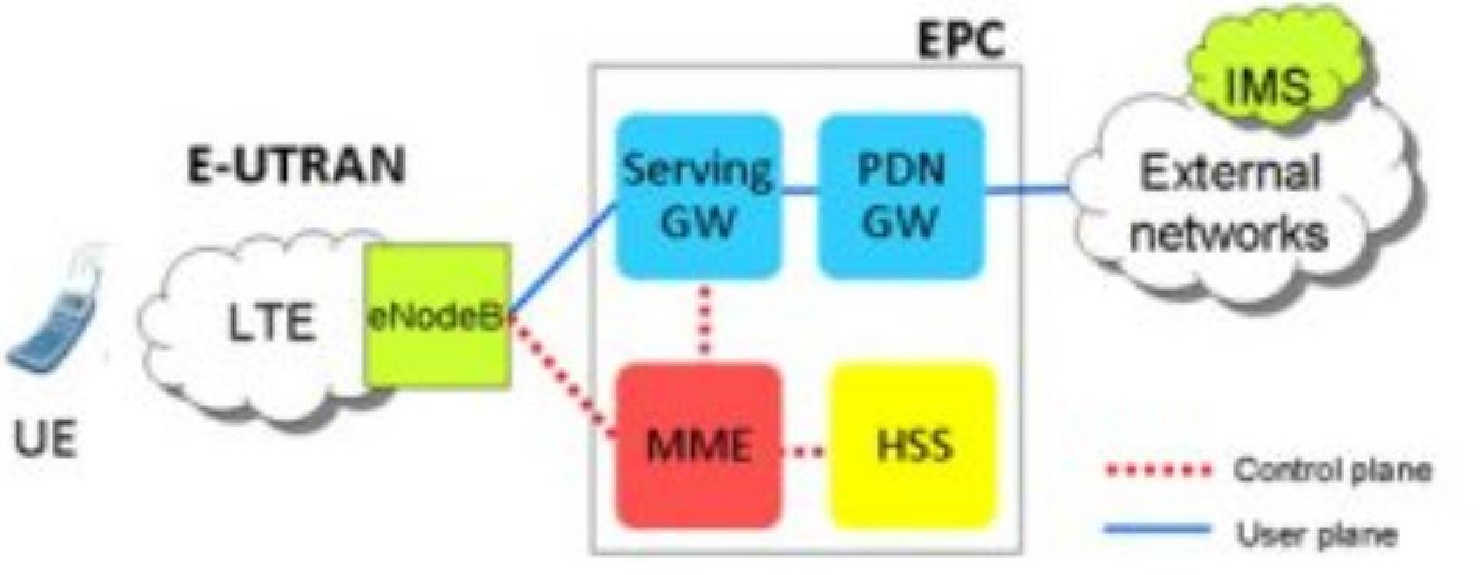
\includegraphics[width=1\linewidth]{LTE_Architektur}
	\caption{Architektur LTE \protect\cite{Fir19}}
	\label{fig:bildarchitektur}
\end{figure}
Die Signalisierungsdaten und die Mediendaten werden separat übermittelt. Die Mediendaten werden der User Plane und die Signalisierungsdaten der Control Plane übergeben. Leitungen verbinden das EPC mit externen Telefonnetzen sowie Datennetzen, dem IP Multimedia Core Network Subsystem (IMS\abk{IMS}{IP Multimedia Core Network Subsystem} , siehe Abb\abk{Abb}{Abbildung} \ref{fig:bildarchitektur}) \cite{Fir19}.
E-UTRAN wird auch Radio Access Network (RAN)\abk{RAN}{Radio Access Network} und das EPC Core Network (CN)\abk{CN}{Core Network} genannt. System Architecture Evolution (SAE) ist der Standard der Architektur von der 3GPP für das CN. LTE und SAE beinhalten das Evolved Packet System (EPS)\abk{EPS}{Evolved Packet System}. Dies bietet eine nahtlose Benutzung des IP vom UE zum Packet Data Network (PDN)\abk{PDN}{Packet Data Network} und gestattet sowohl Quality of Service (QoS)\abk{QoS}{Quality of Service} als auch IP Dienste wie zB VoIP. Es können mehrere Kanäle mit unterschiedlichem QoS von verschiedenen PDN's für unterschiedliche Dienste angeboten werden \cite{Ses11}.
\subsection{Logische Komponenten}
\label{subsec:logkomponenten}
\subsubsection{User Equipment}
\label{subsubsec:ue}
Ab R12 sind der DL und UL in eigenen Kategorien getrennt spezifiziert. Die DL und UL Kategorien können unterschiedlich sein \cite{GPP19}. Das UE ist nicht Teil der zu beschaffenden Infrastruktur. 
\subsubsection{E-UTRAN}
\label{subsubsec:eutran}
Die Architektur im E-UTRAN (siehe Abb. \ref{fig:eutranarchitektur}) ist bewusst flach gehalten und besteht nur aus miteinander über das X2 Protokoll kommunizierenden eNodeB's. Auch die Übergabe von UE an andere eNodeB's regeln diese ressourcenschonend alleine, ohne einen zentralen Controller. Über das S1 Protokoll kommuniziert ein eNodeB mit den CN Knoten. Der Mobility Management Entity (MME)\abk{MME}{Mobility Management Entity} werden die Signalisierungsdaten und dem Serving Gateway (SGW)\abk{SGW}{Serving Gateway} die Mediendaten übergeben. Mit dem S1-flex Protololl versorgen mehrere CN Knoten (MME/S-GWs) eine gemeinsame Region (Pool Area) durch Vernetzung mit den eNodeB's, dem MME/S-GW Pool. Die UE's einer Zelle, die von einem eNodeB betreut werden, sind von mehreren CN-Knoten unterstützt. Das verhindert einen Single Point of Failure bei den CN-Knoten und erlaubt Load Balancing. Der UE Kontext verbleibt normalerweise bei einem MME, solange sich die UE in der selben Pool Area befindet \cite{Ses11}.
\begin{figure}[H]
	\centering
	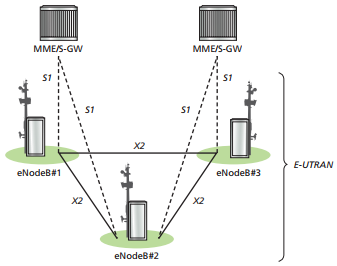
\includegraphics[width=1\linewidth]{images/E_UTRAN_Architektur}
	\caption[]{E-Utran Architektur \protect\cite{Ses11}}
	\label{fig:eutranarchitektur}
\end{figure}
Die Schnittstelle zum UE sind die Access Stratum (AS)\abk{AS}{Access Stratum} Protokolle \cite[S. 131]{Sau06}. Das E-UTRAN ist für das Radio Resource Management (RRM)\abk{RRM}{Radio Resource Management}, also für Funk relevante Funktionen, wie zum Beispiel die Bestimmung der zur Verfügung stehenden Ressourcen  am UE, sowie für die Kompression und Verschlüsselung der Daten, zuständig. Ein UE gehört zu genau einem eNodeB \cite{Ses11}.
\subsubsection{EPC}
\label{subsubsec:epc}
Die wichtigsten logischen Knoten sind:
\begin{itemize}
	\item PDN Gateway (P-GW)
	\item Serving Gateway (S-GW)
	\item Mobility Management Entity (MME)
	\item Home Subscriber Server (HSS)\abk{HSS}{Home Subscriber Server}
	\item Policy Control and Charging Rules Function (PCRF)\abk{PCRF}{Policy Control and Charging Rules Function}
\end{itemize}
Das PCRF ist zuständig für die Policy, also für das Freischalten der Dienste und QoS-Authorisierung, die der Kunde vertraglich mit dem Provider vereinbart hat. Für die Verrechnung wird die PCRF durch die Policy Control Enforcement Function (PCEF) unterstützt. Beide sind physisch in der P-GW untergebracht. Der HSS hingegen enthält das QoS Profil und Zugangsbeschränkungen für das Roaming sowie mögliche PDN's. Die PDN's können mit Access Point Name (APN)\abk{APN}{Access Point Name}, einer Bezeichnung, die den Domain Name System (DNS) Regeln folgen, gekennzeichnet sein. Weiters speichert die HSS den aktuellen MME der UE. Weiters ist das Authentication Center (AUC)\abk{AUC}{Authentication Center} im HSS angesiedelt. Das P-GW verwaltet die IP-Adressen der UE's und ist für die QoS Umsetzung zuständig. Mit Hilfe von Traffic Flow Templates (TFT)\abk{TFT}{Traffic Flow Templates} und den im PCRF hinterlegten Regeln werden unterschiedliche Kanäle mit verschiedenen QoS-Niveaus für unterschiedliche Downlink Kanäle bereitgestellt. Das P-GW ist auch die Schnittstelle zu Netzen mit nicht 3GPP konformen Technologien wie Code-Division Multiple Access 2000 (CDMA2000)\abk{CDMA2000}{Code-Division Multiple Access} und Worldwide Interoperability for Microwave Access (WiMax\,\textsuperscript{\tiny\textregistered})\abk{WiMax\,\textsuperscript{\tiny\textregistered}}{Worldwide Interoperability for Microwave Access}. Alle User IP-Pakete gehen durch das S-GW, welches als Puffer für die unterschiedlichen Kanäle dient, wenn das UE sich zwischen den eNodeB's wechselt. Auch wenn das UE im Ruhezustand ist werden mit Unterstützung des EPS Connection Management--IDLE (ECM-IDLE)\abk{ECM-IDLE}{EPS Connection Management — IDLE}  Downlink Daten und Kanalinformationen gespeichert. Das S-GW speichert auch Metadaten für die Verrechnung wie zB Downloadvolumen und ist für die Lawful Interception zuständig. Ebenso ist es die Schnittstelle zu 3GPP Technologien wie General
Packet Radio Service (GPRS)\abk{GPRS}{General
Packet Radio Service} oder Universal Mobile Telecommunications System (UMTS)\abk{UMTS}{Universal Mobile Telecommunications System}. Die MME ist verantwortlich für die Signalisierung zwischen UE und CN. Die Protokolle nennt man Non Access Stratum (NAS)\abk{NAS}{Non Access Stratum} und regeln das Kanal und Verbindungsmanagement. Sobald das UE im Netz eingeschaltet wird, erhält es vom MME eine SAE Temporary Mobile Subscriber Identity (S-TMSI)\abk{S-TMSI}{SAE Temporary Mobile Subscriber Identity}, die dem UE Kontext zugeordnet ist. Der Kontext enthält zB die vom HSS heruntergeladenen Profilinformationen. Die MME ist auch für die Security wie zB Authentifizierung verantwortlich. Um die Kosten zu senken und die Ansprechzeit zu erhöhen werden die Daten gecached. Dynamisch werden Daten von aufgebauten Verbindungen und Terminal Daten gespeichert. Ist das UE im Ruhezustand (ECM-IDLE state) wird der Kontext, auch RAN-Daten, dauerhaft gesichert. Dazu sendet das UE beim Verlassen der Tracking Area (TA)\abk{TA}{Tracking Area} ein Tracking Area Update. Die MME ist für die Lokalisierung einer UE im Ruhezustand verantwortlich. Sind Downlink Informationen für eine UE verfügbar, werden alle eNodeB's im aktuellen TA von der MME informiert. Der eNodeB in der aktuellen Zelle verständigt die UE, welche sich durch eine Service Request Procedure in den ECM-CONNECTED State versetzt, was idle-to-active transition genannt wird. Danach baut die MME eine Verbindung auf. Um diesen Prozess zu beschleunigen, arbeiten NAS und AS Protokolle wenn möglich gleichzeitig \cite{Ses11}.

%\subsubsection{Roaming}
%\label{subsubsec:etxterne}
%Ein Netzwerk, das von einem Operator in einem Land betrieben wird, heißt Public Land Mobile Network (PLMN)\abk{PLMN}{Public Land Mobile Network}. Befindet sich die UE in einem fremden PLMN verbindet sich diese mit dem lokalen E-UTRAN. Dieses verbindet sich mit dem lokalen MME und S-GW. Die MME autorisiert über die heimatlichen HSS die Signalisierung und die S-GW leitet nach erfolgreichem Nachfragen bei der heimatlichen P-GW den Medienstrom weiter (siehe%\abk{Abb}{Abbildung}\ref*{fig:roaming})
%Abb\abk{Abb}{Abbildung} \ref{fig:roaming}\cite{Ses11}).
%\begin{figure}[H]
%	\centering
%	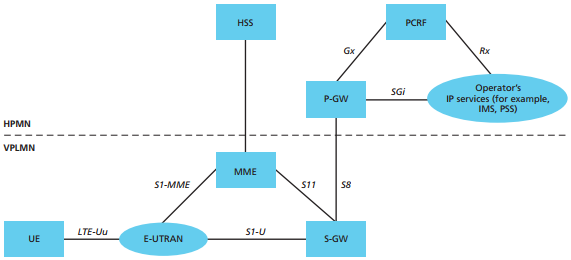
\includegraphics[width=1\linewidth]{images/Roaming}
%	\caption{Roaming Architektur \protect\cite{Ses11}}
%	\label{fig:roaming}
%\end{figure}




%----------------------------------------------------------------
%
%  File    :  komponenten.tex
%
%  Authors :  ???
% 
%  Created :  7 Sept 2019
% 
%  Changed :  7 Sept 2019
% 
%---------------------------------------------------------------


\section{Komponenten}
\label{sec:Komponenten}
	\subsection{Use Cases}
	\label{subsec:Use Cases}
	
	Aufgrund der Tatsache dass, sich das 4G LTE Mobilfunknetz über verschiedene Sektoren wie dem Öffentlichen Dienst, der Energieversorgung, dem Transportwesen, wie auch dem Bildungsbereich sowie auch dem Gesundheitswesen erstrecken soll, ergeben sich als Anforderungen vor allem eine hohe Abdeckung, sowie hohe Datenraten, welche für die Benutzer, also die Inselbewohner, verfügbar sein sollen \cite{Tch18}. 

Zusätzlich verfügt die zu betrachtende Insel über ein Seenotrettungssystem, präziser gesagt ein maritimes Rettungs-Koordinationszentrum, über welches mit Hilfe von Rettungsschiffen und Rettungsdrohnen in Seenot geratene Inselbewohner lokalisiert werden können \cite{eckermann2018tinylte}. Des Weiteren bewegen sich die Einwohner auf dem Staatsgebiet der Insel in autonom fahrenden Autos, weshalb auch hierfür entsprechende Anforderungen in Bezug auf die Komponenten für vehikulare Kommunikation bei der Planung eines Mobilfunknetzes berücksichtigt werden sollte. Da eine Infrastruktur von Grund auf erbaut wird, muss keine Rücksicht auf etwaige bestehende Legacy Architekturen genommen werden, in welche neue Komponenten zu integrieren sind. 
\subsection{State of the Art Marktanalyse}
\label{subsec:Marktanalyse}

Um die ansäßigen Inselbewohner zufrieden zustellen, sollten insbesondere Peak Data Raten, die Zellkapazitäten, der Zellradius, die Radio Access Modi, die Antennen Schemata, sowie das Mobility Speed Handover konkreter in Erwägung gezogen werden\cite{Dat14}.
Bei der Recherche zur Thematik haben sich folgende Kriterien als Unterscheidungsmerkmale herauskristallisiert, welche eine Entscheidungsfindung beeinflussen. Ob nun anhand dieser letztlich eine Entscheidung getroffen wird, ob nun ein Mobilfunknetz selbst errichtet (Make) oder die notwendigen Komponenten (Buy) hinzugekauft werden sollen, wird im Kapitel Make or Buy näher beleuchtet. Neben dem Spektrum, dem Durchsatz (Throughput), der Latenz (Latency), der Redundanz (Redundancy), der Interoperabilität beziehungsweise der Kompatibilität, ist auch die Möglichkeit der Skalierbarkeit, um etwaige Nachbarinseln mitzuversorgen, von signifikanter Bedeutung. Denn diese haben ihrerseits kooperativ ihre Hilfe zur Analyse der Problematik in Form der Nutzung eines Internet Cafes angeboten, um erste Recherchearbeit bezüglich des Aufbaus eines LTE Mobilfunknetzes zu liefern. Zusätzlich  als weitere nicht zu vernachlässigende Elemente stellen auch Kriterien wie das des Monitorings respektive des Control Managements, ebenso wie dem möglichen Coverage, als auch die Kapazität Faktoren dar, welche die finalen Entscheidungsprozesse maßgeblich beeinflussen. Zudem sollte abzuwägen sein, ob ein "Easy to use enerprise Dashboard" vorhanden ist. Des Weiteren wird wichtig zu prüfen, ob Lincesing an für sich eine Problematik darstellen könnte. Inwiefern auf der Südsee Insel nach internationalem Recht bzw. in welchen gesetzlichen Rahmenbedingungen die Verantwortlichen Projektleiter sich bewegen und dementsprechend danach handeln.
	\subsection{Anbieter am Markt}
	\label{subsec:Anbieter am Markt}
	Eine Vielzahl von Anbietern für die Errichtung eines Mobilfunknetzes bestimmen derzeit den globalen LTE Advanced Markt.\ Die dominierenden Unternehmen an diesem sind neben Ambra Solutions, Arris International,
	Athonet, Cisco, Comba, DruidSoftware, Ericsson, Future Technologies, General Dynamics und 
	Huawei. Neben diesen existieren aber auch weitere Anbieter wie beispielsweise Lemko, Luminate Wireless,
	Mavenir,
	NEC,
	Netnumber,
	Nokia,
	Pdvwireless,
	Quortus,
	Redline Communications,
	Samsung,
	Sierra Wireless,
	Star Solutions,
	Ursys,
	Verizon und 
	Zinwave \cite{Max19}.
	Abhängig von den Use Cases ergeben sich bei der Analyse und beim Design spezifizierte funktionale wie auch Nicht-funktionale Anforderungen. Durch die konkrete Betrachtung einer Einführung eines Mobilfunknetzes gilt es, sich mit auftretenden Fragestellungen wie  dem Angebot an qualifiziertem Fachpersonal, welches auf den LTE Advanced Standard geschult ist, auseinander zu setzen. Dieses kann dann sowohl in den Phasen der Analyse und des Designs als auch in denen der Implementierung sowie bei Wartung und beim Testen vor Inbetriebnahme gezielt eingesetzt werden. Ist entsprechendes Kapital vorhanden, eine Armada externer Berater einzufliegen, die schon einmal ähnliche Projekte realisiert haben, um mit Hilfe derer Erfahrungswerte von vergangenen Projekten in Bezug auf Planung, Koordination und Aufwandsabschätzungen zu nutzen und somit Fehleinschätzungen zu minimieren im ideal Fall zu vermeiden. Sind generell Fachkräfte mit domain spezifischem Know-How verfügbar oder ist es sinnvoll Schulungszentren aufzubauen, um langfristig Abhängigkeiten von Schulungsdienstleistern zu verringern.
%	\subsection{HSS, EPC, PCRF}
%	\label{subsec:Antennen HSS, EPC, PCRF}
%		\subsection{Preise der Komponenten}
%	\label{subsec:Preise der Komponenten}
	\subsection{Antennen Konfigurationen}
	\label{subsec:Antennen Konfigurationen}
Bevor man die Komponenten, welche von unterschiedlichen Marktteilnehmern angeboten werden vergleicht, ist es durchaus sinnvoll ein Bild über die Empfangsbedingungen in dem Inselstaat machen. Abhängig von physikalischen Einflussfaktoren in Form von Waldgebieten, Gebäudekomplexen oder topologischen Strukturen wie Gebirge sie darstellen, können ebensolche signifikant die Signalübertragung bestimmen. Denn schließlich sind Absorption, Beugung oder auch Reflexion mit die Hauptgründe für Störungen bei der Ausbreitung elektromagnetischer Wellen. Um nun einen optimalen Empfang zu gewähren kann eine Kombination aus Antennentypen angedacht werden, da jede einzelne Bauart ihre Vor- und Nachteile aufweist. So ist zu unterscheiden zwischen Mono- und Breitband Antennen. Mono-Antennen sind hierbei der Klasse der Richtantennen und Breitbandantennen der Klasse der Rundstrahler zuzuordnen. \cite{Sch19}
\begin{figure*}[ht]
	\centering
	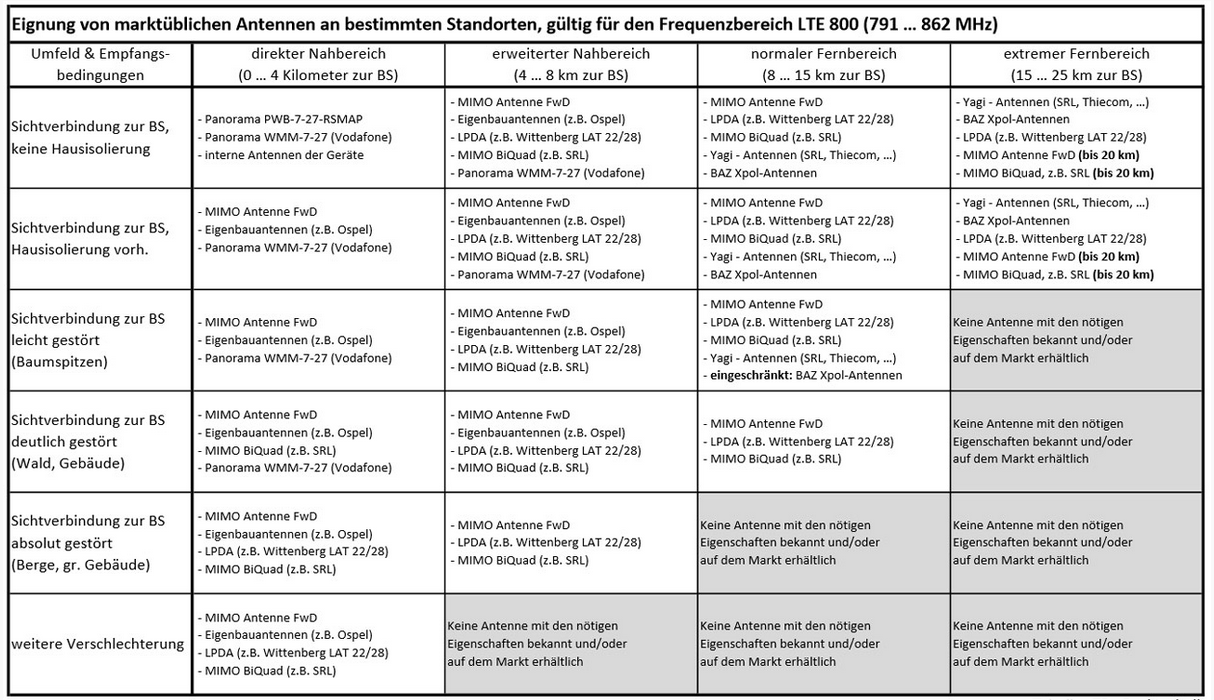
\includegraphics[width=1\linewidth]{images/tabellemcnantennen}
	\caption{Antennenüberblick  \protect\cite{Sch19}}
	\label{fig:tabellemcnantennen}
\end{figure*}

%\newpage
 %\flushbottom 
%\nextpage
\raggedbottom 


%\newpage

%----------------------------------------------------------------
%
%  File    :  open_source.tex
%
%  Authors :  ???
% 
%  Created :  7 Sept 2019
% 
%  Changed :  7 Sept 2019
% 
%---------------------------------------------------------------

\section{Open Source Lösung}
\label{sec:open_source}

Im Gegenzug zu teurer Spezial-Hardware und nicht frei zugänglicher Software, gibt es auch sogenannte Open-Source Lösungen. Grundsätzlich kann eine Software als Open-Source bezeichnet werden, wenn der Quellcode dieser veröffentlicht wird. Im Gegenzug, zur einfachen Bereitstellung einer rein ausführbaren Datei.
Des Weiteren wird frei zugängliche Software oftmals mit eingeschränkten, oder keinen Beschränkungen weitergegeben. Diese ist daher oftmals frei und kostenlos zu verwenden und somit auch erweiter- und veränderbar. \cite{gacek2004many}

\subsection{OpenAirInterface - OAI}
Im konkreten Anwendungsfall, ermöglicht es eine solche Software, kostengünstig ein eigenes LTE-Netzwerk aufzubauen. 
Ganz ohne Hardware geht dies natürlich nicht, jedoch würde ein Modul für etwa 1500,- ausreichen um ein entsprechendes Netz aufzubauen. Ein solches Software Defined Radio (SDR) wäre etwa das "Flexible, next-generation, open source software-defined radio"\ von LimeMicrosystems, welches im Zuge einer Crowdfunding-Aktion realisiert wurde \cite{CroudLime01}. 

Mit einem SDR werden Anteile der Signalverarbeitung mittels Software realisiert. Dies kann von dedizierter Hardware unterstützt werden. Des Weiteren bietet es eine gewisse Flexibilität zu einer reiner Hardware Lösung, da Software veränderbar ist \cite{jondral2005software}. 

Das OpenAirInterface ist ein Projekt der OpenAirInterfaceTM Software Alliance (OSA), welches eine Open Source Lösung zur Verfügung stellt \cite{OpenAir19}.

Dabei wird die Lösung in zwei Projekte unterteilt. 
\begin{itemize}
	\item eNodeB (eNB): “openairinterface5G”
	\item evolved packet core (EPC): “openair-cn”
\end{itemize}

OpenAirInterface ist die erste Open-Source Software Platform welche eines LTE Systems welches den vollen Protokollstack des 3GPP Standards, inklusive E-UTRAN und EPC unterstützt.
Dabei kann dies sowohl für das Erstellen eines eigenen LTE Netzes, als auch das Überwachen (Monitoring) verwendet werden \cite{nikaein2014openairinterface}.
Des Weiteren ist es möglich, Performance-Analysen durchzuführen und dabei Einblicke zu erhalten, wie sich ein rasch skalierendes System verhält. 

\begin{figure*}[ht]
	\centering
	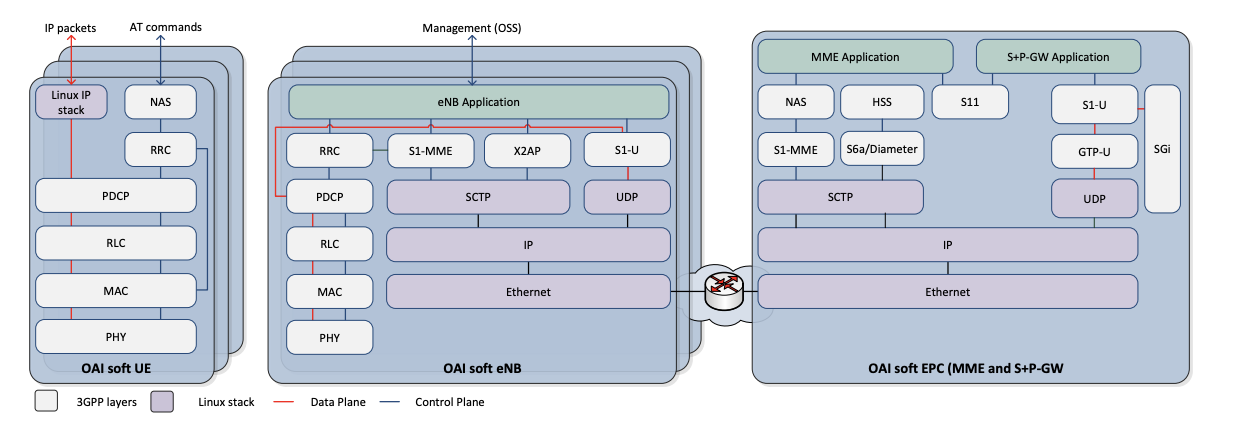
\includegraphics[width=1.025\linewidth]{BestandTeileOAI}
	\caption{Übersicht LTE Module in den jeweiligen Projekten \protect\cite{openAirInterfaceOverview19}}
	\label{fig:modulesOAI}
\end{figure*}


Abbildung \ref{fig:modulesOAI} zeigt die schematische Implementierung des LTE Protokoll Stacks in OAI.
Dem Hersteller zufolge wurden hiermit auch diverse Tests durchgeführt. So wurde Beispielsweise OAI eNB mit kommerziellen Huawei Geräten getestet, bei welchen LTE aktiviert wurde (E392, E398u-1) und OAI-UE mit CMW500 (Ericsson on com4Innov network).

Die OpenAirInterface Open Source Initiative bietet sowohl Unterstützung für eNodeB (eNB), User Equipment (UE) wie auch Evolved Packet Core (EPC) an. Zudem wird, neben dem oben erwähnten Lime SDR auch noch ETTUS  USRP und ExpressMIMO2 unterstützt. Des Weiteren erlaubt OAI hierbei auch die Unterstützung kommerzieller Ausrüstung \cite{kaltenberger2019openairinterface}. Somit ist man hier nicht auf ein spezielles SDR eingeschränkt.

\subsection{srsLTE}
srsLte bietet eine sehr modulare Architektur, um auch rasch neue Standards einfließen lassen zu können. Diese ist in funktionale Module aufgebaut. Damit wird hier auch bereits ein Satz an Beispielanwendungen geboten, welche für eigene Anwendungen angepasst werden können \cite{puschmann2017implementing}. 
Des Weiteren sind auch Anpassungen möglich, um zusätzliche Hardware zu unterstützen. 
Abbildung \ref{fig:modulessrsLTE} zeigt diesen modularen Aufbau.

\begin{figure*}[ht]
	\centering
	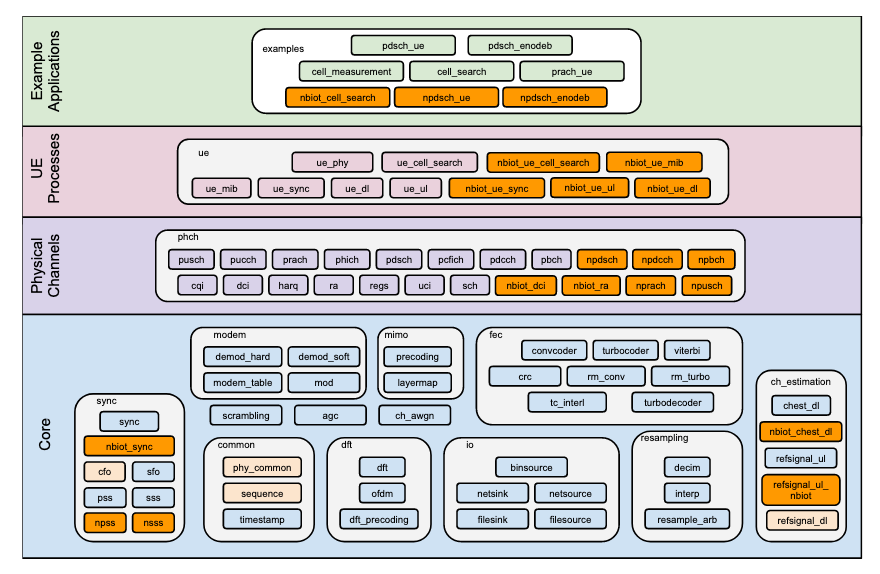
\includegraphics[width=1.015\linewidth]{ssrLTE_Module}
	\caption{Übersicht Architektur srsLTE \protect\cite{puschmann2017implementing}}
	\label{fig:modulessrsLTE}
\end{figure*}

Die Beispielanwendungen geben einen Überblick zum Betrieb als eNodeB (srsENB, srsEPC) sowie Informationen um dies als UE (srsUE) einsetzen zu können. Entwickelt wurde diese von Software Radio Systems, welche dieses Projekt auf Github zur Verfügung stellt \cite{githubSrSLTE}.

Die hohe Flexibilität und Anpassbarkeit ist auch Grund für Abwandlungen und andere Projekte, welches dies srsLTE als Basis verwenden. So ist etwa \nameref{tinyLTE} eines dieser genannten Projekte. Zudem wird die Software regelmäßig gewartet, was auch an den Codeänderungen im Repository zu erkennen ist. 

\subsection{tinyLTE}
\label{tinyLTE}
Eine weitere Open-Source Lösung ist tinyLTE. Auch dieses verwendet SDR, um größtmögliche Flexibilität und Offenheit zu bieten. Dabei unterstützt dies sowohl als LTE Client (UE) als auch Infrastruktur (eNB + EPC) \cite{eckermann2018tinylte}.

Der Vorteil dabei ist, dass hiermit ein gleichzeitiger Betrieb von beiden Anwendungsfällen möglich ist. In Kombination mit Hardware, welches 2 SDRs unterstützt, kann so ein einzelnes Gerät die volle Funktionalität anbieten. 
Beides basiert, mit geringen Änderungen, auf srsLTE \cite{gomez2016srslte}. 

Die Lösung von Philipp Gorczak sowie Fabian Eckermann wurde auf Github zur Verfügung gestellt. Eine Evaluierung im Betrieb wurde ebenfalls bereits getestet. Dabei ging es um die Kommunikation über LTE zwischen Fahrzeugen. 

\subsection{Unterschiede}
Alle drei erwähnten Lösungen bieten einen breiten Funktionsumfang und Unterstützung an. Unterschiede sind etwa in der getesteten Hardware zu erkennen. Sollte bereits bestehendes Equipment vorhanden sein, könnte dies ein Indikator für eine Präferenz darstellen. 
tinyLTE wurde speziell für die Kommunikation zwischen Fahrzeugen entwickelt und getestet. 
%\newpage

%----------------------------------------------------------------
%
%  File    :  make_buy.tex
%
%  Authors :  ???
% 
%  Created :  7 Sept 2019
% 
%  Changed :  7 Sept 2019
% 
%---------------------------------------------------------------

\section{Make or Buy}
\label{sec:make_buy}

Kosten und Preise wurden nicht ermittelt. Die erwähnten Anbieter haben kaum Preise öffentlich ausgeschrieben, welche vergleichbar sind. Kosten variieren, je nach Umfang und tatsächlich eingesetzter Hardware, stark. Grundsätzlich ist jeglicher aktuelle Service erwerbbar und hängt von dem Budget ab, welches ausgegeben wird.

Die Kosten der Open-Source Variante liegen in der Umsetzung und dem Testen. Der Vorteil besteht darin, dass diese an beliebige Bedürfnisse angepasst werden kann. In diesem Fall ist, verglichen mit proprietären Anbietern, mehr Geld für Schulungen, Aufbau von Know-How und Wartung aufzuwenden. 

Der Aufbau des Know Hows kann zudem genutzt werden, um ein proprietäres Produkt inklusive Dienstleistungen zu erzeugen. So ist es möglich, diese später zu verwenden, um bei der LTE Anbindung anderer Inseln zu unterstützen und die Initialkosten zu senken. Auch die Errichtung eines Ausbildungszentrums ist denkbar.

Ein Nachteil dieser Lösung ist, dass ein Sicherheitsfaktor besteht. Im Problemfall kann kein externer Anbieter zur Verfügung gezogen werden, welcher dieses System wartet und das Problem behebt. Dies ist Teil der Verträge mit proprietären Anbietern.

\subsection{Entscheidungsbegründung}
Für den Fall der Anbindung anderer Systeme, oder dem Zusammenführen von weiteren Systemen, bieten die Open Source Lösungen bereits eine gute Unterstützung. Ausweitungen auf weitere Inseln kann daher, ohne Festlegung auf einen speziellen Anbieter, durchgeführt werden.

Eine funktionsfähiges LTE Netzwerk wird, sofern dies von einem proprietären Anbieter umgesetzt wird, schneller zur Verfügung stehen. Grund hierfür ist, dass es keinen Einarbeitungsaufwand gibt und die Umsetzung von Fachpersonal durchgeführt wird, wodurch auch die Kosten steigen.
Des Weiteren ist das Risiko des Scheiterns, bei einem völlig selbst entwickelten Netzwerks, höher.

Trotz der aufgeführten Nachteile, ist eine Umsetzung mittels Open Source Lösung zu präferieren. Diese ist preisgünstig umzusetzen. Ein Umstieg auf einen etablierten Anbieter kann auch später erfolgen, sollte es zu nicht überwindbaren Problemen kommen.

%\subsection{Kriterien für Make or Buy Entscheidung}


%\subsubsection{Differenzierung der Antennenleistung}
%\subsubsection{Testbarkeit}


%\subsubsection{Begründung}
%\newpage

%----------------------------------------------------------------
%
%  File    :  make_buy.tex
%
%  Authors :  ???
% 
%  Created :  7 Sept 2019
% 
%  Changed :  7 Sept 2019
% 
%---------------------------------------------------------------

\section{Sicherheit}
\label{sec:sicherheit}
\subsection{Kritische Infrastrukturen}
Um die Inselbewohner vor Wirtschaftsspionage, Diebstahl und Manipulation zu schützen, ist die Thematik der Sicherheit konsequenterweise nicht zu vernachlässigen. Da Cyber-Kriminelle heutzutage sehr professionell agieren, um ihr Schadensausmaß möglichst maximal zu gestalten, sind die kritischen Infrastrukturen (KI) der Inseleinrichtungen wie z.B. die Energieversorgung und Kommunikationssysteme von Spitälern besonders zu schützen. Um zur politischen und sozialen Stabilität auf der Insel beizutragen, sind somit Versorgungsengpässe beziehungsweise das Risiko von Ausfällen in KI zu reduzieren. Denn Beeinträchtigungen in diesen Bereichen können zu kaskadierenden Effekten in anderen Lebensbereiche führen. Die Digitalisierung der Insel erfordert besondere Schutzmaßnahmen, sodass durch Prävention, Detektion und Reaktion für sowohl dem Staat, der heimischen Wirtschaft und eben auch der Gesellschaft trotz zunehmender IT-Abhängigkeit und -Vernetzung auch in Zukunft zuverlässig KIs funktionieren\cite{BSI17}.

Laut Bundesamt für Sicherheit in der Informationstechnik (BSI) sind potentielle Gefährdungen im Zusammenhang mit öffentlichen Mobilfunknetzen bei der Planung und Errichtung vor allem Wartung ebendieser nicht außer Acht zu lassen. Ebenso sollten mögliche Gegenmaßnahmen in Erwägung gezogen werden, um den Schutz konfidenzieller Daten erhöhen zu können \cite{Ger08}.
\subsection{Sicherheitsgefährdungen und Schutzmaßnahmen}
Erfolgt ein Zugriff auf die implementierten technischen Einrichtungen kann dies zu Missbrauch durch Unbefugte führen. Dies kann geschehen zum Einen durch Schwachstellen bei Endgeräte-Authentisierung, potenzielle Schwachstelle in der Datenverschlüsselung, durch unzureichende Verschlüsselungsstärke, Erstellung von Bewegungsprofilen durch Ortung, Unterbindung von Mobilfunkkommunikation durch Störsender oder Software-Manipulation der UE. Um nur auf einige von vielen Sicherheitsgefährdungen wie z.B. Over-The-Air Programming (OTA), einzugehen, Proxy-Manipulation, FOTA – Firmware Over The Air oder mangelnde Implementierung von Sicherheitsmechanismen. Mögliche Schutzmaßnahmen dienen zur Prüfung von Software-Abhängigkeiten oder dem Einfordern von Sicherheitszertifizierungen. 
Betrachtet man Übertragungsverfahren, Datenübertragungsraten sowie weitere Technologien im Bereich von Mobilfunknetzen, ist zu verzeichnen, dass zwar die Sicherheitsrisiken wesentlich komplexer wurden gleichzeitig paradoxerweise das Bewusstsein der Nutzer allerdings nicht in gleichem Ausmaß angestiegen ist. Aus diesem Grund kann es durchaus nützlich sein, dieses Bewusstsein dezidierter zu schärfen\cite{Ger08}.

\subsection{Regelungen für Telekommunikationsunternehmen}

Da sich unter den Inselbewohnern auch IT-versierte Juristen befinden, wurde ein IT-Sicherheitsgesetz erlassen, welches die Telekommunikationsunternehmen verpflichtet, die IT Infrastrukturen nach dem Stand der Technik angemessen abzusichern. In einem Zyklus von Minimum alle 24 Monate muss die Sicherheit geprüft werden.
Des weiteren besteht eine Verpflichtung der Anbieter gegenüber den Inselbewohnern, diese zu warnen, sofern es Grund zur Annahme gibt, das die UE für IT-Angriffe missbraucht wurden. Zusätzlich herrscht eine Informationspflicht dahingehend, dass auf möglichst viele Arten hingewiesen wird, wie etwaige Störungen zu entfernen sind.
Natürlich sollen IT-Sicherheitsmaßnahmen nicht nur zum Schutz von personenbezogenen Daten der Inselbewohner, sondern auch zum Schutz vor unerlaubten Eingriffen in die Infrastruktur eingesetzt werden.
Auch zu beachten ist, das auftretende IT-Sicherheitsvorfälle gemeldet werden bei den zuständigen Behörden.\cite{BSI17}  


%----------------------------------------------------------------
%
%  File    :  conclusion.tex
%
%  Authors :  ???
% 
%  Created :  7 Sept 2019
% 
%  Changed :  7 Sept 2019
% 
%---------------------------------------------------------------

\section{Conclusion}
\label{sec:conclusion}
\subsection{Zusammenfassung der Ergebnisse}
\label{subsec:zusammenfassung}
Lorem Ipsum is simply dummy text of the printing and typesetting industry. Lorem Ipsum has been the industry's standard dummy text ever since the 1500s, when an unknown printer took a galley of type and scrambled it to make a type specimen book. It has survived not only five centuries, but also the leap into electronic typesetting, remaining essentially unchanged. It was popularised in the 1960s with the release of Letraset sheets containing Lorem Ipsum passages, and more recently with desktop publishing software like Aldus PageMaker including versions of Lorem Ipsum.
\subsection{Ausblick}
\label{subsec:ausblick}
Lorem Ipsum is simply dummy text of the printing and typesetting industry. Lorem Ipsum has been the industry's standard dummy text ever since the 1500s, when an unknown printer took a galley of type and scrambled it to make a type specimen book. It has survived not only five centuries, but also the leap into electronic typesetting, remaining essentially unchanged. It was popularised in the 1960s with the release of Letraset sheets containing Lorem Ipsum passages, and more recently with desktop publishing software like Aldus PageMaker including versions of Lorem Ipsum.







% if have a single appendix:
%\appendix[Proof of the Zonklar Equations]
% or
%\appendix  % for no appendix heading
% do not use \section anymore after \appendix, only \section*
% is possibly needed

% use appendices with more than one appendix
% then use \section to start each appendix
% you must declare a \section before using any
% \subsection or using \label (\appendices by itself
% starts a section numbered zero.)
%

%Anhang
\appendices
%Abkuerzungsverzeichnis
\printnomenclature
\label{app:abkuerzungen}


% references section

% can use a bibliography generated by BibTeX as a .bbl file
% BibTeX documentation can be easily obtained at:
% http://mirror.ctan.org/biblio/bibtex/contrib/doc/
% The IEEEtran BibTeX style support page is at:
% http://www.michaelshell.org/tex/ieeetran/bibtex/
\bibliographystyle{IEEEtran}
\bibliography{reif_fuer_die_insel_jrnl}
\label{app:literatur}
%\bibliography{../bib/reif_fuer_die_insel_jrnl.bbl}
% argument is your BibTeX string definitions and bibliography database(s)
%\bibliography{IEEEabrv,../bib/paper}
%
% <OR> manually copy in the resultant .bbl file
% set second argument of \begin to the number of references
% (used to reserve space for the reference number labels box)

%\begin{thebibliography}{1}

%\bibitem{IEEEhowto:kopka}
%H.~Kopka and P.~W. Daly, \emph{A Guide to \LaTeX}, 3rd~ed.\hskip 1em plus
%  0.5em minus 0.4em\relax Harlow, England: Addison-Wesley, 1999.
%\end{thebibliography}

% biography section
% 
% If you have an EPS/PDF photo (graphicx package needed) extra braces are
% needed around the contents of the optional argument to biography to prevent
% the LaTeX parser from getting confused when it sees the complicated
% \includegraphics command within an optional argument. (You could create
% your own custom macro containing the \includegraphics command to make things
% simpler here.)
%\begin{IEEEbiography}[{\includegraphics[width=1in,height=1.25in,clip,keepaspectratio]{mshell}}]{Michael Shell}
% or if you just want to reserve a space for a photo:

\end{document}


